%%%%%%%%%%%%%%%%%%%%%%%%%%%%%%%%%%%%%%%%%
% Short Sectioned Assignment
% LaTeX Template
% Version 1.0 (5/5/12)
%
% This template has been downloaded from:
% http://www.LaTeXTemplates.com
%
% Original author:
% Frits Wenneker (http://www.howtotex.com)
%
% License:
% CC BY-NC-SA 3.0 (http://creativecommons.org/licenses/by-nc-sa/3.0/)
%
%%%%%%%%%%%%%%%%%%%%%%%%%%%%%%%%%%%%%%%%%

%----------------------------------------------------------------------------------------
%	PACKAGES AND OTHER DOCUMENT CONFIGURATIONS
%----------------------------------------------------------------------------------------

\documentclass[paper=a4, fontsize=11pt]{scrartcl} % A4 paper and 11pt font size

\usepackage{ctex}
\usepackage{amssymb}
\usepackage{listings}
\usepackage[T1]{fontenc} % Use 8-bit encoding that has 256 glyphs
\usepackage{fourier} % Use the Adobe Utopia font for the document - comment this line to return to the LaTeX default
\usepackage[english]{babel} % English language/hyphenation
\usepackage{amsmath,amsfonts,amsthm} % Math packages

\usepackage{lipsum} % Used for inserting dummy 'Lorem ipsum' text into the template

\usepackage{sectsty} % Allows customizing section commands
%\allsectionsfont{\centering \normalfont\scshape} % Make all sections centered, the default font and small caps

\usepackage{fancyhdr} % Custom headers and footers
\usepackage{algorithm}
\usepackage[noend]{algpseudocode}
\usepackage{subcaption}
\graphicspath{{p3/}}
%\usepackage{algorithmic}
\usepackage[noend]{algpseudocode}
\usepackage{listings}
\pagestyle{fancyplain} % Makes all pages in the document conform to the custom headers and footers
\fancyhead{} % No page header - if you want one, create it in the same way as the footers below
\fancyfoot[L]{} % Empty left footer
\fancyfoot[C]{} % Empty center footer
\fancyfoot[R]{\thepage} % Page numbering for right footer
\renewcommand{\headrulewidth}{0pt} % Remove header underlines
\renewcommand{\footrulewidth}{0pt} % Remove footer underlines
\setlength{\headheight}{13.6pt} % Customize the height of the header

\numberwithin{equation}{section} % Number equations within sections (i.e. 1.1, 1.2, 2.1, 2.2 instead of 1, 2, 3, 4)
\numberwithin{figure}{section} % Number figures within sections (i.e. 1.1, 1.2, 2.1, 2.2 instead of 1, 2, 3, 4)
\numberwithin{table}{section} % Number tables within sections (i.e. 1.1, 1.2, 2.1, 2.2 instead of 1, 2, 3, 4)

\setlength\parindent{0pt} % Removes all indentation from paragraphs - comment this line for an assignment with lots of text

%----------------------------------------------------------------------------------------
%	TITLE SECTION
%----------------------------------------------------------------------------------------

\newcommand{\horrule}[1]{\rule{\linewidth}{#1}} % Create horizontal rule command with 1 argument of height

\title{	
\normalfont \normalsize 
%\textsc{university, school or department name} \\ [25pt] % Your university, school and/or department name(s)
\horrule{0.5pt} \\[0.4cm] % Thin top horizontal rule
\huge Analysis and Design of Algorithm - Homework 4\\ % The assignment title
\horrule{2pt} \\[0.5cm] % Thick bottom horizontal rule
}

\author{宁雪妃} % Your name
%\author{Xuefei Ning} % Your name

\date{\normalsize\today} % Today's date or a custom date

\begin{document}

\maketitle % Print the title

%----------------------------------------------------------------------------------------
%	PROBLEM 1
%----------------------------------------------------------------------------------------

\section{书面作业}

% \section{}
% \lipsum[2] % Dummy text
\textbf{15.1-4. 修改MEMOIZED-CUT-ROD, 使之不仅返回最优收益值, 还返回切割方案}

修改如下:
\begin{algorithm}[ht]
  \caption{MEMOIZED-CUT-ROD(p, n)}
  \begin{algorithmic}[1]
  \State $r[0..n], s[0..n] = new array$
  \State $i = 0$
  \For{$i = 0 .. n$}
  \State $ r[i] = -1$
  \State $ s[i] = -1$
  \EndFor
  \State $profit = MEMOIZED-CUT-ROD-AUX(p, n, r, s)$
  \State $plan = []$
  \State $x = n$
  \While{$x \neq s[x]$}
  \State $plan.append(s[x])$
  \State $x = x - s[x]$
  \EndWhile
  \State $plan.append(x)$
  \State\Return $profit, plan$
  \end{algorithmic}
\end{algorithm}

\begin{algorithm}[ht]
  \caption{MEMOIZED-CUT-ROD-AUX(p, n, r, s)}
  \begin{algorithmic}[1]
    \If{$r[n] \geq 0$}
    \Return $r[n]$
    \EndIf
    \If{$n == 0$}
    \State $q = 0$
    \Else
    \For{$i=1..n$}
    \State $newq = MEMOIZED-CUT-ROD-AUX(p, n-i, r, s)$
    \If{$newq > q$}
    \State $q = newq$
    \State $s[n] = i$
    \EndIf
    \EndFor
    \EndIf
    \State $r[n] = q$
    \State\Return q
  \end{algorithmic}
\end{algorithm}
加入了数组S, 其中每个元素S[i]代表长度为i的钢条的第一刀应该怎么切才能够使利益最大化。
\\[4ex]
% --------

\textbf{15.3-4. 使用动态规划方法, 我们首先求解子问题, 然后选择哪些子问题用来构建原问题的最优解。Capulet教授认为, 我们不必为了求原问题最优解而总是求出所有的子问题。她建议, 在求矩阵链乘法问题的最优解时, 我们总是可以在求解子问题之前选定$A_iA_{i+1} \dots A_j$的划分位置$A_k$(选定的$k$使得$p_{i-1}p_kp_j$最小)。请找出一个反例, 证明这个贪心算法可能产生次优解。}

如果使用该贪心算法, 相当于每次找到的划分位置$k$都是在满足$p_k = min(p_i ... p_{j-1})$的。想要举出这个贪心算法的反例, 先来看一下最简单的需要划分的情况, 比如三个矩阵进行乘法的情况: $A_0A_1A_2$, 其中$A_i \in R^{p_i \times p_{i+1}}$。不失一般性, 假设$p_1 < p_2$, 那么贪心算法会选择$p_1$作为第一个分界点, 这种选择使得整体要做的乘法次数为$T_1 = p_0p_1p_3 + p_1p_2p_3$; 如果选择$p_2$作为分界点, 乘法次数为$T_2 = p_0p_2p_3 + p_0p_1p_2$。只需要找到某个$p_0, p_1, p_2, p_3$的配置使得$T_1 > T_2$即是该算法最优的反例。即:
\[
p_0p_1p_3 + p_1p_2p_3 > p_0p_2p_3 + p_0p_1p_2 \implies p_0p_3(p_2-p_1) < p_1p_2(p_3-p_0)
\]
满足上式且$p_2 > p_1, p_3 > p_0$的配置肯定存在, 因为两边的形式对称, 要么$p_0p_3(p_2 - p_1) \equiv p_1p_2(p_3-p_0)$, 这个显然不成立。那么就一定能构造出使任何一边小的取值, 比如我们尝试$p_2 = 3, p_1 = 2; p_3 = 4, p_0 = 1$, 此时得到$p_0p_3(p_2-p_1) = 4 < p_1p_2(p_3-p_0)=18$, $T_1 = 8 + 24 = 32 > T_2 = 12 + 6 = 18$, 举出反例, 该算法可能生成次优解。(反例只需要一次尝试一定能够构造出来, 因为如果发现尝试的解使得$T_1$ < $T_2$, 只需要交换$p_2, p_1$和$p_3, p_0$的取值组合即可)。
\\[4ex]
% --------

\textbf{证明可能的线裁剪个数为m的指数函数}

以第$m$行每个点为结尾可能的线裁剪个数$l_{m, i}$满足$2^m < l_{m, i} < 3^m$, 总的线裁剪个数满足$n2^m < l_{m, *} < n3^m$。其中$2^m$的极端情况是考虑一个在图片边缘上的像素$a_{i, 0}$, 以这个像素为结尾的线个数为$l_{i, 0} = l_{i-1, 0} + l_{i-1, 1}$。事实上这个松下界可以进一步放紧, 考虑计算以第$i$行元素为结尾的线个数$l_{i, *}$, 有$l_{i, *} = 3 \times l_{i-1,*} - l_{i-1,0} - l_{i-1,n-1} \geq 3 \times l_{i-1,*} - \frac{2}{n}l_{i-1,*} = (3-\frac{2}{n})l_{i-1,*}$, 即$l_{m-1, *}\geq (3-\frac{2}{n})^{m-1}n$。由上可知$\mbox{num}$为一个$m$ 的指数函数。

\section {线裁剪实验报告}

\subsection{开发平台}

\begin{itemize}
\item 平台: Mac OS X 10.11.2
\item Python 2.7.10
\item 依赖库: python-opencv(用于读图); numpy==1.8.2
\end{itemize}

\subsection{运行方法}

运行:
\begin{lstlisting}[language=bash]
  python seam_carving.py <输入图片名>
\end{lstlisting}
结果图片将写入运行目录下的\textbf{out\_输入文件名}文件。

\subsection{算法描述}
本次实验中使用动态规划的方法进行图像裁剪, 一次线裁剪的问题定义为: 从每行(列)中去掉一个像素(且为了保证去掉这个像素不会影响图像的连续性, 每行(列)去掉的像素必须连续(也就是在行(列)方向相差)最多一个像素), 使得去掉后对整体图像的语义效果(内容)影响最小。对于语义效果的定义并不明确, 但是在某个定义下, 可以定义每条线的cost为"这条线上所有像素与周边像素的差别之和最小"。

这个问题显然可以用动态规划解决, 以列方向的线裁剪(即从每行移除一个像素)为例, 可以简单的将原问题看为两步:
\begin{enumerate}
\item 求以最后一行的任意一个元素$a_{n-1,i}$为结尾的线中最小代价的线$l_{n-1, i}$.
\item 对于这张图, 裁剪的最小cost为: $\min_{i=0}^{n-1} cost(l_{n-1, i})$.
\end{enumerate}

对于第一步, 可以用动态规划求解:
\begin{enumerate}
\item 定义较小规模的子问题: 规模为$i$的子问题$Q_{i,j}$为: 求解以$i$行$j$列的元素为结尾的裁剪线$l_{i,j}$。
\item 从小规模$i$的子问题合成规模为$i+1$的问题: 对于$Q_{i+1,j}$, $cost(l_{i,j}) = \min_{\delta=-1}^{\delta=1}{cost(i, j + \delta)} + d(i, j)$, 同时$j$加上对应的$\delta$即为$l_{i+1,j}$这条线在第$i$行的列坐标。
\end{enumerate}
从问题规模为0的问题自底向上构建该表格, 设原图大小为$m \times n$。每行子问题的计算需要$\Theta(n)$, 总复杂度为$\Theta(mn)$。

作业要求中要求将原图裁剪到$\frac{m}{2} x \frac{n}{2}$。如果用线裁剪方法, 算法复杂度为$\Theta(mn^2) + \Theta(nm^2) = \Theta(mn(m+n))$。

进行一次列方向线裁剪的动态规划算法如~\ref{algorithm:3}所示, 其中$\mbox{im}$为大小为$m \times n$的输入图片, $d(im, x, y)$为该图片的第$x$行第$y$列像素的cost。
\begin{algorithm}[ht]
  \caption{SEAM-CARVING(im, m, n, d)}
  \label{algorithm:3}
  \begin{algorithmic}[1]
    \State $cost\_mat = new matrix(m, n),\quad initialize -\infty$
    \State $way\_mat = new matrix(m - 1, n)$
    \For{$x = 0 .. n-1$}
    \State $cost\_mat[0, x] = d(im, 0, x)$
    \EndFor
    \For{$y = 1 .. m-1$}
    \For{$x = 0 .. n-1$}
    \For{$\delta = -1 .. 1$}
    \If $(y, x + \delta)在图像中$
    \If $cost\_mat[y-1, x+\delta] > cost\_mat[y,x]$
    \State $cost\_mat[y,x] = cost\_mat[y-1, x+\delta] + d(im, y, x)$
    \State $way\_mat[y-1, x] = x + \delta$
    \EndIf
    \EndIf
    \EndFor
    \EndFor
    \EndFor

    \State $way=[(m-1, \mbox{arg}\min(cost\_mat[m-1, :]))]$
    \For {$y = m-1 .. 1$}
    \State $way.append((y-1, way[-1] + way\_mat[y-1, way[-1]]))$
    \EndFor
    \State $\mbox{reverse}(way)$
    \State $\mbox{remove all the pixels in `way`}$
  \end{algorithmic}
\end{algorithm}

\subsection{实验效果}
下面是一个将原大小为$250 \times 201$的图片经过多次线裁剪, 得到大小为$125 \times 100$的图片的结果~\ref{pic:1}。使用的每个像素的cost函数$d$为和两边像素的均方差, 也尝试了使用每个像素和四周像素的均方差作为$d$, 效果相差无几。
\begin{figure}
  \centering%
  \subcaptionbox{}[4cm]
                {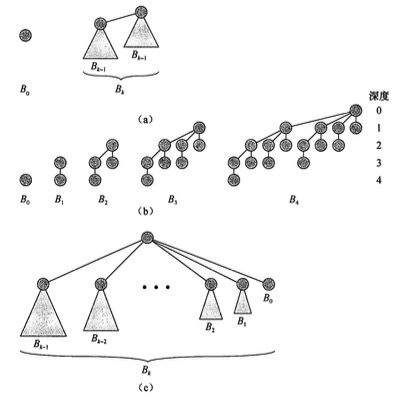
\includegraphics[height=3cm]{1}}
                %\hspace[3cm]%
                \subcaptionbox{}[4cm]
                              {\includegraphics[height=3cm]{out_1}}
                              \caption{效果示意图1}
                              \label{pic:1}
\end{figure}


\end{document}
